\documentclass[11pt,a4paper,oneside]{article}
\usepackage[latin1]{inputenc}
\usepackage{amsmath}
\usepackage{amsfonts}
\usepackage{amssymb}
\usepackage{graphicx}
\usepackage{color}
\usepackage {tikz}
\usepackage{fancyvrb}
\usetikzlibrary {er}
\usepackage[left=2.00cm, right=2.00cm, top=1.00cm]{geometry}
\graphicspath{{./}}
\fvset{tabsize=4}

\begin{document}
	\title{DS 221 - Introduction to Scalable Systems \\ Parallel Merge Sort using MPI}
	\author{Shriram R. \\ M Tech (CDS) \\ 06-02-01-10-51-18-1-15763}
	\maketitle
	
	\section{Introduction}
    Parallel Merge Sorting algorithm has been implemented using MPI and the speedup for different number of processes with respect to sequential version were observed through experiments. The following sections cover the methodology, experimental setup and results in detail.
	
	\section{Methodology}
	The parallel version of the algorithm performs the following steps:
	\begin{enumerate}
		\item The input data is read in from the file by process 0. File I/O has been used to read input instead of shell redirection to improve performance 
		\item Process 0 divides the input equally among the processes and sends the respective chunks to other processes. If input is not divisible exactly, last process would get some additional data items
		\item Each process receives its chunk of data and stores it in a local array. The length of data is also captured in a variable
		\item Each process performs a local quick sort on its chunk of data. Quick sort has been implemented as a seperate function in the program for this purpose.
		\item The merging of data happens in a tree-like fashion as given below for the specific case of 8 processes,
		
		\begin{center}
			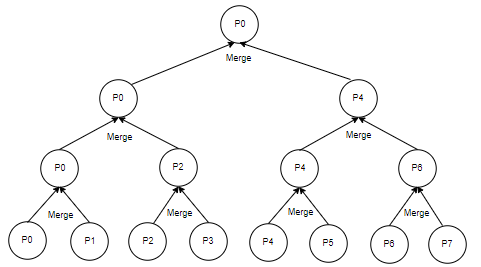
\includegraphics[scale=1.0]{3.png}		
		\end{center}		
				
	\end{enumerate}
    The final sorted data will be available in process 0 and is written to stdout. The above methodology is illustrated in a code snippet in the appendix.
    
    \begin{verbatim}
       
    \end{verbatim}
	
	
	\section{Experimental Setup}
	Experiments were run on multiple compute nodes having 8 core AMD Opteron 3380 processor in the Turing compute cluster. Batch jobs were created in the form of a shell script and executed using PBS. The no. of nodes used varied depending on the no. of processes required for the experiment.\\
	\newline
	The time taken to run the parallel sort was measured using C library functions and was printed to stdout along with specified output. Each experiment was repeated 20 times consecutively and then the average was computed for the plots and analysis. \\
	\newline
	In each experiment, both sequential and parallel versions of code were executed so as to remove bias from any system load. \\
	
	\section{Results}
	
	The experimental results are tablulated and plotted below,
	
	  \begin{center}
		\begin{tabular}{|c|c|c|c|}
			\hline 
			\textbf{Processes}  & \textbf{Sequential (Avg.) (s)} & \textbf{Parallel (Avg.) (s)} & \textbf{Speedup} \\
			\hline
		    8 &  0.0311 & 0.0065 & 4.82\\ 
			\hline 
		    16 &  0.0324 & 0.0534 & 0.62\\
			\hline 
			32 &  0.0319 & 0.0.0662 & 0.48\\
			\hline 
			64 &  0.0330 & 0.1444 & 0.23\\ 
			\hline 
			80 &  0.0351 & 0.4512 & 0.08 \\
			\hline  
		\end{tabular}
	\end{center}
	\begin{verbatim}
	
	\end{verbatim}
	\begin{center}
		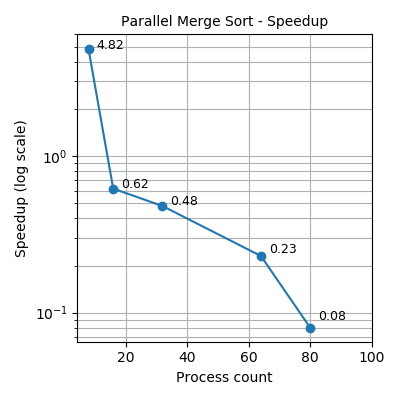
\includegraphics[scale=0.7]{4.png}		
	\end{center}

     \begin{verbatim}
             
     
     
     \end{verbatim}
    \section{Observations}
    It can be observed that the speedup is maximum for 8 processes which corresponds to 8 cores in a single node and then decreases with increase in process count. \\
    \newline
    As the process count is increased, the processes are distributed across multiple nodes. This leads to more delay in data transfer and synchronization due to communication across different nodes through the network. Therefore, the parallel version performs worser than the sequential code for higher process count. \\
    \newline
    The speedup is also heavily dependent on the CPU load in the nodes. At the time of experiments, only one node had a very low CPU load and all the other nodes were overutilized with load averages close to 100. This could have contributed to decrease in speedup as well. \\
       
    
    \section{References}
    \begin{list}{}{}
    	\item 1. https://en.cppreference.com/w/c
    	\item 2. DS 221 Course lecture notes
    	\item 3. http://www.arc.ox.ac.uk/content/how-run-mpi-applications
    	\item 4. https://www.open-mpi.org/faq/?category=running
    	\item 5. https://www.open-mpi.org/doc/v2.1/man1/mpiexec.1.php
    \end{list}

    \section{Appendix - Code} 
    
    \begin{Verbatim}
    // Send and Receive Input
    if (rank == 0) {
    	for (int i = 1; i < procs; i++) {
    		if (i < procs - 1)
    			MPI_Send(arr + i * (SIZE / procs), SIZE / procs, MPI_INT, i, 0, comm);
    		else
    			MPI_Send(arr + i * (SIZE / procs), SIZE - i * (SIZE / procs), MPI_INT,
    																	  i, 0, comm);
    	}
    	len = SIZE / procs;
    } else {
    	MPI_Recv(arr, SIZE, MPI_INT, 0, 0, comm, &status);
    	MPI_Get_count(&status, MPI_INT, &len);
    }
    
    // Perform local quick sort
    qusort(arr, 0, len - 1);
    
    
    
    
    
    
    // Perform Merge
    step = 0;
    while (1 << step < procs) {
    	if ((rank + 1) % (2 << step) == 1 && rank + (1 << step) < procs) {
    		MPI_Recv(arr2, SIZE, MPI_INT, rank + (1 << step), step, comm, &status);
    		MPI_Get_count(&status, MPI_INT, &len2);
			merge(arr, len, arr2, len2, temp);
    		p = arr;
    		arr = temp;
    		temp = p;
    		len += len2;
    	} else if ((rank + 1) % (2 << step) != 1) {
    		// printf("Send %d %d \n", step, rank);
    		MPI_Send(arr, len, MPI_INT, rank - (1 << step), step, comm);
    		break;
    	}
    	step++;
    }
    
    MPI_Barrier(comm);
    
    \end{Verbatim}
    
\end{document}